\documentclass{article}
\usepackage[a4paper,left=1cm,right=1cm,top=2cm,bottom=1cm]{geometry}

\usepackage{fancyhdr}
%\pagestyle{empty}
%\thispagestyle{fancy}
%\pagestyle{fancy}
\renewcommand{\headrulewidth}{0pt}
\renewcommand{\footrulewidth}{0pt}
\fancyhf{}
\fancyhead[C]{
\includegraphics[height=1cm]{Logos/logo_MPSA.jpg} \quad 
\includegraphics[height=1cm]{Logos/logoIREM.jpg}
\hfill
%{\small Groupe \og{}Faire de l'informatique sans ordinateur à l'école et au collège\fg{}}

\includegraphics[height=.5cm]{Logos/iso-crop.pdf}
\hfill \begin{minipage}{2.4 cm}
\begin{center}

\includegraphics[height=.5cm]{Logos/by-nc-sa-eu.png}
\\
\small f\'evrier 2020
\end{center}
\end{minipage}
}
\fancyfoot[R]{
}
\fancyfoot[L]{
}
\fancyfoot[C]{
%\thepage
}



% \usepackage{lscape}
\usepackage[utf8]{inputenc}
%\usepackage[title,titletoc,toc]{appendix}
%\usepackage{listings,multicol}
\usepackage{amsmath}
\usepackage{amssymb}
% \usepackage{amsthm}
%\usepackage{hyperref}
\usepackage{mathtools}
\usepackage{float}
\usepackage{caption}
\usepackage{wrapfig}
\usepackage{stmaryrd}
%\usepackage[ruled,vlined,linesnumbered]{algorithm2e}
%\usepackage{xspace}
\usepackage{subfig}
%\usepackage{pgfplotstable}
%\usepackage{pgfplots}
%\usepackage{fancyref}
\usepackage{caption}
\usepackage{scratch3}
%\usepackage{galois}
%\usepackage{fancybox}
%\renewcommand{\floatpagefraction}{.8}%

%\setlength{\belowcaptionskip}{-0.6cm}
% \setlength{\abovecaptionskip}{0cm}

\setscratch{else word=else}

\newcommand\textbox[1]{%
  \parbox{.31\textwidth}{#1}%
}
\newcommand\textboxx[1]{%
  \parbox{.47\textwidth}{#1}%
}

\newenvironment{allowbreaks}
{\mathactivatecomma
  \mathcode`\,=\string"8000
  \ignorespaces}
{\ignorespacesafterend}

\newcommand{\mathactivatecomma}{%
  \begingroup\lccode`~=`\,
  \lowercase{\endgroup\edef~}{\mathchar\the\mathcode`\,\penalty0 }}


\newcommand*{\eg}{e.g.\@\xspace}
\newcommand\myeq{\stackrel{\mathclap{\normalfont\mbox{\tiny$\Delta$}}}{=}}

\newcommand*{\todo}{\textbf{\color{red} TODO}}
% sharpify
\newcommand\sh[1]{#1^{\sharp}}
% sharpify and prime
\newcommand\shp[1]{#1^{\sharp \prime}}
\newcommand\shpp[1]{#1^{\sharp \prime \prime}}

% Post
\newcommand\pp{\mathbf{Post}}

% Summary
\newcommand\su{\mathbf R}

%_v
\newcommand\vv[1]{#1_{\mathcal V}}

% keywords
\newcommand\kw[1]{\emph{\textcolor{orange}{#1}}}
\newcommand\kww[1]{\mathbf{\textcolor{scarletred}{#1}}}

% Variables
%% a variable
\newcommand\var{v}
%% a set of variable
\newcommand\svar{\mathfrak V}
%% the set of all variables
\newcommand\savar{\mathcal V}

% Function
%% a function
\newcommand\fun{f}
%% a set of function
\newcommand\sfun{\mathfrak F}
%% the set of all function
\newcommand\safun{\mathcal F}

% Expressions
%% an expression
\renewcommand\exp{e}
%% a set of expression
\newcommand\sexp{\mathcal E}
%% the set of all expressions
\newcommand\saexp{\kw{expr}}

% Statements
%% set of all statements
\newcommand\sastmt{\kw{stmt}}
%% a set of statement
\newcommand\sstmt{\mathcal S}
%% a statement
\newcommand\stmt{\texttt{stmt}}

% Programs
%% set of all programs
\newcommand\saprgm{\kw{prgm}}
%% a set of programs
\newcommand\sprgm{\mathcal P}
%% a program
\newcommand\prgm{p}
% Left values
%% set of all left-values
\newcommand\salv{\kw{lval}}
%% a left-value
\newcommand\lv{lv}

% cells
%% set of all cells
\newcommand\sacell{\mathcal{C}ell}
%% a set of cells
\newcommand\scell{C}
%% a cell
\newcommand\ocell{c}
\newcommand\mopsa{\textsc{Mopsa}}


% expression operations
%% dereferences
\newcommand{\deref}{\texttt{*}}
%% addressing
\newcommand{\addof}{\texttt{\&}}

% set of definition
\newcommand{\defset}{\mathbf{def}}
\newcommand{\codef}{\overline{\mathbf{def}}}

\makeatletter
\newenvironment{CenteredBox}{% 
\begin{Sbox}}{% Save the content in a box
\end{Sbox}\centerline{\parbox{\wd\@Sbox}{\TheSbox}}}% And output it centered
\makeatother

\usepackage{scalerel}
\DeclareMathOperator*{\bigcircledast}{\scalerel*{\circledast}{\sum}}

\newcommand\rc[1]{\mathbf{#1}}
\newcommand\cell[3]{\langle #1 , #2, #3 \rangle}
\newcommand\eval[2]{\mathbb E \llbracket #1 \rrbracket (#2)}
\newcommand\aeval[2]{\mathbb E^{\sharp} \llbracket #1 \rrbracket (#2)}
\newcommand\exec[2]{\mathbb S \llbracket #1 \rrbracket (#2)}
\newcommand\aexec[2]{\mathbb S^{\sharp} \llbracket #1 \rrbracket (#2)}
\newcommand\aeexec{\sh{\mathbb{S}}_{\mathbf R}}
\newcommand\aeexecapp[2]{\sh{\mathbb{S}}_{\mathbf R}\llbracket #1 \rrbracket(#2)}

\newcommand{\ad}{\texttt{@}}
\newcommand\saad{\mathcal A}
\newcommand\oad{\mathfrak a}

\newcommand\tdot[1]{\tikz{\fill[#1] circle(3pt);}}

\newcommand\chdefset[2]{#1_{\mid #2}}
\renewcommand\v[1]{\ovalvariable{#1}}
\renewcommand\o[1]{\ovaloperator{#1}}
\newcommand\num[1]{\ovalnum{#1}}

\newcommand\saml{\mathfrak V}
\newcommand\dsaml{\mathfrak V^{\star}}
\newcommand{\splitatcommas}[1]{%
  \begingroup
  \begingroup\lccode`~=`, \lowercase{\endgroup
    \edef~{\mathchar\the\mathcode`, \penalty0 \noexpand\hspace{0pt plus 1em}}%
  }\mathcode`,="8000 #1%
  \endgroup
}
%\input{lst.tex}
%\input{tikz.tex}

\begin{document}

\pagestyle{empty}
\thispagestyle{fancy}
\rotatebox{90}{
\scalebox{.95}{
  \begin{tikzpicture}[scale=3]
    \draw (0, 0) rectangle (9, 6.3);
    \draw (0, 0) rectangle (3, 3.15);
    \draw (0, 3.15) rectangle (0.5, 2.65);
    \node[] at (0.25,2.90) {\texttt{E2}};
    \draw[->,very thick] (0,1.575) -- (0.5,1.575);
    \draw (3, 3.15) rectangle (3, 6.3);
    \draw (0, 6.30) rectangle (0.5, 5.80);
    \node[] at (0.25,6.05) {\texttt{E1}};
    \draw[->,very thick] (0,4.725) -- (0.5,4.725);
    \draw (3, 0) rectangle (6, 2.1);
    \draw (3, 6.30) rectangle (3.5, 5.80);
    \node[] at (3.25,6.05) {\texttt{A}};
    \draw (3, 2.1) rectangle (6, 4.2);
    \draw (3, 4.2) rectangle (3.5, 3.7);
    \node[] at (3.25,3.95) {\texttt{B}};
    \draw (3, 4.2) rectangle (6, 6.3);
    \draw (3, 2.1) rectangle (3.5, 1.6);
    \node[] at (3.25,1.85) {\texttt{C}};
    \draw (6, 0) rectangle (9, 3.15);
    \draw (6, 3.15) rectangle (6.5, 2.65);
    \node[] at (6.25,2.90) {\texttt{S2}};
    \draw (6, 0) rectangle (9, 3.15);
    \draw (6, 6.3) rectangle (6.5, 5.80);
    \node[] at (6.25,6.05) {\texttt{S1}};
    \draw[-,very thick] (8.5,4.725) -- (9,4.725);
    \draw[-,very thick] (8.5,1.575) -- (9,1.575);
  \end{tikzpicture}
}
}
  \newpage
~
\newpage

\thispagestyle{fancy}

\rotatebox{90}{ 
\scalebox{.95}{
  \begin{tikzpicture}[scale=3]
    \draw (0, 0) rectangle (9, 6.3);
    \draw (0, 0) rectangle (3, 3.15);
    \draw (0, 3.15) rectangle (0.5, 2.65);
    \node[] at (0.25,2.90) {\texttt{E2}};
    \draw[->,very thick] (0,1.575) -- (0.5,1.575);
    \draw (3, 3.15) rectangle (3, 6.3);
    \draw (0, 6.30) rectangle (0.5, 5.80);
    \node[] at (0.25,6.05) {\texttt{E1}};
    \draw[->,very thick] (0,4.725) -- (0.5,4.725);
    \draw (3, 0) rectangle (6, 2.1);
    \draw (3, 6.30) rectangle (3.5, 5.80);
    \node[] at (3.25,6.05) {\texttt{A}};
    \draw (3, 2.1) rectangle (6, 4.2);
    \draw (3, 4.2) rectangle (3.5, 3.7);
    \node[] at (3.25,3.95) {\texttt{B}};
    \draw (3, 4.2) rectangle (6, 6.3);
    \draw (3, 2.1) rectangle (3.5, 1.6);
    \node[] at (3.25,1.85) {\texttt{C}};
    \draw (6, 0) rectangle (9, 3.15);
    \draw (6, 3.15) rectangle (6.5, 2.65);
    \node[] at (6.25,2.90) {\texttt{S2}};
    \draw (6, 0) rectangle (9, 3.15);
    \draw (6, 6.3) rectangle (6.5, 5.80);
    \node[] at (6.25,6.05) {\texttt{S1}};
    \draw[-,very thick] (8.5,4.725) -- (9,4.725);
    \draw[-,very thick] (8.5,1.575) -- (9,1.575);
  \end{tikzpicture}
}}
  
\newpage
~
\newpage

\thispagestyle{fancy}
 \rotatebox{90}{ 
 \scalebox{.95}{
  \begin{tikzpicture}[scale=3]
    \draw (0, 0) rectangle (9, 6.3);
    \draw (0, 0) rectangle (3, 3.15);
    \draw (0, 3.15) rectangle (0.5, 2.65);
    \node[] at (0.25,2.90) {\texttt{E2}};
    \draw[->,very thick] (0,1.575) -- (0.5,1.575);
    \draw (3, 3.15) rectangle (3, 6.3);
    \draw (0, 6.30) rectangle (0.5, 5.80);
    \node[] at (0.25,6.05) {\texttt{E1}};
    \draw[->,very thick] (0,4.725) -- (0.5,4.725);
    \draw (3, 0) rectangle (6, 2.1);
    \draw (3, 6.30) rectangle (3.5, 5.80);
    \node[] at (3.25,6.05) {\texttt{A}};
    \draw (3, 2.1) rectangle (6, 4.2);
    \draw (3, 4.2) rectangle (3.5, 3.7);
    \node[] at (3.25,3.95) {\texttt{B}};
    \draw (3, 4.2) rectangle (6, 6.3);
    \draw (3, 2.1) rectangle (3.5, 1.6);
    \node[] at (3.25,1.85) {\texttt{C}};
    \draw (6, 0) rectangle (9, 3.15);
    \draw (6, 3.15) rectangle (6.5, 2.65);
    \node[] at (6.25,2.90) {\texttt{S2}};
    \draw (6, 0) rectangle (9, 3.15);
    \draw (6, 6.3) rectangle (6.5, 5.80);
    \node[] at (6.25,6.05) {\texttt{S1}};
    \draw[-,very thick] (8.5,4.725) -- (9,4.725);
    \draw[-,very thick] (8.5,1.575) -- (9,1.575);
  \end{tikzpicture}
}}
  
\newpage
~
\newpage


\thispagestyle{fancy}
  
\begin{tabular}{cc}
  \resizebox{.5\textwidth}{!}{
  \begin{scratch}
    \blockinit{quand \v{E1} est présent}
    \blockvariable{mettre \v{S1} à \o{\v{E1}+\num{1}}}
%    \blockstop{stop}
  \end{scratch}
  }
  &
    \begin{minipage}{0.5 \textwidth}
      \vspace{4 cm}
      \hfill \scalebox{2}{\LARGE{\textsc{Incrément}}} \hfill~
    \end{minipage}
\end{tabular}

\begin{tabular}{cc}
  % % \begin{figure}[h!]
  % %   \centering
  \resizebox{.5\textwidth}{!}{

  \begin{scratch}
    \blockinit{quand \v{E1} est présent}
    \blockvariable{mettre \v{S1} à \v{E1}}
    \blockvariable{mettre \v{S2} à \v{E1}}
%    \blockstop{stop}
  \end{scratch}
  }
  &
    \begin{minipage}{0.5 \textwidth}
      \vspace{8 cm}
      \hfill \scalebox{2}{\LARGE{\textsc{Photocopie}}} \hfill~
    \end{minipage}
\end{tabular}

\newpage
~
\newpage

\thispagestyle{fancy}
\begin{tabular}{cc}
  \resizebox{.5\textwidth}{!}{
  \begin{scratch}
    \blockinit{quand \v{E1} et \v{E2} sont présents}
    \blockvariable{mettre \v{A} à \v{E1}}
    \blockvariable{mettre \v{B} à \v{E2}}
    \blockvariable{mettre \v{C} à \ovalnum{0}}
    \blockrepeat{répéter jusqu'à \o{\v{A}=\v{B}}}
    {
      \blockvariable{mettre \v{C} à \o{\v{C}+\num{1}}}
      \blockvariable{mettre \v{A} à \o{\v{A}-\num{1}}}
    }
    \blockvariable{mettre \v{S1} à \v{C}}
    \blockvariable{mettre \v{S2} à \num{0}}
%    \blockstop{stop}
  \end{scratch}
  }
  &
    \begin{minipage}{0.5 \textwidth}
      \vspace{8 cm}
      \scalebox{2}{\LARGE{\textsc{Moins}}}\\      
     (condition $E1>E2$)
    \end{minipage}
\end{tabular}
\newpage
~
\newpage

\thispagestyle{fancy}
\begin{tabular}{cc}
  \resizebox{.5\textwidth}{!}{
  \begin{scratch}
    \blockinit{quand \v{E1} et \v{E2} sont présents}
    \blockvariable{mettre \v{A} à \v{E1}}
    \blockvariable{mettre \v{B} à \v{E2}}
    \blockvariable{mettre \v{C} à \ovalnum{0}}
    \blockrepeat{répéter jusqu'à \o{\v{A}=\v{B}}}
    {
      \blockvariable{mettre \v{C} à \o{\v{C}+\num{1}}}
      \blockvariable{}
    }
    \blockvariable{mettre \v{S1} à \v{C}}
    \blockvariable{mettre \v{S2} à \num{0}}
%    \blockstop{stop}
  \end{scratch}
  }
  &
    \begin{minipage}{0.5 \textwidth}
      \vspace{8 cm}
       \scalebox{2}{\LARGE{\textsc{\textsc{Moins$^{\star}$}}}}\\
      (Condition $E1>E2$)
    \end{minipage}
\end{tabular}

\newpage
~
\newpage

\thispagestyle{fancy}

\begin{tabular}{cc}
  \resizebox{.5\textwidth}{!}{
  \begin{scratch}
    \blockinit{quand \v{E1} est présent}
    \blockvariable{mettre \v{A} à \v{E1}}
    \blockrepeat{répéter jusqu'à \o{\v{A}=\num{0}}}
    {
      \blockvariable{mettre \v{A} à \o{\v{A}+\num{1}}}
    }
     \blockvariable{mettre \v{S1} à \v{A}}
%    \blockstop{stop}
  \end{scratch}
  }
  &
    \begin{minipage}{0.5 \textwidth}
      \vspace{8 cm}
      \hfill \scalebox{2}{\LARGE{\textsc{Super}}} \hfill~
    \end{minipage}
\end{tabular}
\newpage
~
\newpage

\thispagestyle{fancy}

\begin{tabular}{cc}
  % % \begin{figure}[h!]
  % %   \centering
  \resizebox{.5\textwidth}{!}{
  \begin{scratch}
    \blockinit{quand \v{E1} est présent}
    \blockvariable{mettre \v{A} à \num{1}}
    \blockifelse{si \o{\v{E1}=Arrêt} alors}
    {
      \blockrepeat{répéter jusqu'à \o{\v{A}=\num{0}}}
      {
        \blockvariable{mettre \v{A} à \o{\v{A}+\num{1}}}
      }
    }
    {
      \blockvariable{mettre \v{S1} à \num{0}}
      \blockvariable{mettre \v{S2} à \num{0}}
    }
%    \blockstop{stop}
  \end{scratch}
  }
  &
    \begin{minipage}{0.5 \textwidth}
      \vspace{8 cm}
      \hfill \scalebox{2}{\LARGE{\textsc{Négation}}} \hfill~
    \end{minipage}
\end{tabular}
\newpage
~
\newpage

\thispagestyle{fancy}
% 
\begin{tabular}{cc}
  % % \begin{figure}[h!]
  % %   \centering
  \resizebox{.5\textwidth}{!}{

  
  \begin{scratch}
    \blockinit{quand \v{E1} et \v{E2} sont présents}
    \blockifelse{si \boolsensing{l'exécution de \v{E1} se termine sur l'entrée  \v{E2}} alors}
    {
      \blockvariable{mettre \v{S1} à \num{Arrêt}}
      \blockvariable{mettre \v{S2} à \num{0}}
    }
    {
      \blockvariable{mettre \v{S1} à \num{Non Arrêt}}
      \blockvariable{mettre \v{S2} à \num{0}}
    }
%    \blockstop{stop}

  \end{scratch}
  }
  &
    \begin{minipage}{0.5 \textwidth}
      \vspace{8 cm}
      \hfill \scalebox{2}{\LARGE{\textsc{Halt}}} \hfill~
    \end{minipage}
\end{tabular}

\newpage
~
\newpage


\thispagestyle{fancy}

\scalebox{0.4}{
  \begin{tabular}{cc}
    % % \begin{figure}[h!]
    % %   \centering
    \resizebox{.5\textwidth}{!}{
    \begin{scratch}
      \blockinit{quand \v{E1} est présent}
      \blockvariable{mettre \v{S1} à \o{\v{E1}+\num{1}}}
%      \blockstop{stop}
    \end{scratch}
    }
    &
      \begin{minipage}{0.5 \textwidth}
        \vspace{4 cm}
        \hfill \scalebox{2}{\LARGE{\textsc{Incrément}}} \hfill~
      \end{minipage}
  \end{tabular}
} \scalebox{0.4}{
  \begin{tabular}{cc}
    % % \begin{figure}[h!]
    % %   \centering
    \resizebox{.5\textwidth}{!}{
    \begin{scratch}
      \blockinit{quand \v{E1} est présent}
      \blockvariable{mettre \v{S1} à \o{\v{E1}+\num{1}}}
%      \blockstop{stop}
    \end{scratch}
    }
    &
      \begin{minipage}{0.5 \textwidth}
        \vspace{4 cm}
        \hfill \scalebox{2}{\LARGE{\textsc{Incrément}}} \hfill~
      \end{minipage}
  \end{tabular}
}

\scalebox{0.4}{
  \begin{tabular}{cc}
    % % \begin{figure}[h!]
    % %   \centering
    \resizebox{.5\textwidth}{!}{
    \begin{scratch}
      \blockinit{quand \v{E1} est présent}
      \blockvariable{mettre \v{S1} à \o{\v{E1}+\num{1}}}
%      \blockstop{stop}
    \end{scratch}
    }
    &
      \begin{minipage}{0.5 \textwidth}
        \vspace{4 cm}
        \hfill \scalebox{2}{\LARGE{\textsc{Incrément}}} \hfill~
      \end{minipage}
  \end{tabular}
} \scalebox{0.4}{
  \begin{tabular}{cc}
    \resizebox{.5\textwidth}{!}{
    \begin{scratch}
      \blockinit{quand \v{E1} est présent}
      \blockvariable{mettre \v{A} à \v{E1}}
      \blockrepeat{répéter jusqu'à \o{\v{A}=\num{0}}}
      {
        \blockvariable{mettre \v{A} à \o{\v{A}+\num{1}}}
      }
%      \blockstop{stop}
    \end{scratch}
    }
    &
      \begin{minipage}{0.5 \textwidth}
        \vspace{8 cm}
        \hfill \scalebox{2}{\LARGE{\textsc{Super}}} \hfill~
      \end{minipage}
  \end{tabular}
}

% \scalebox{0.4}{
% \begin{tabular}{cc}
%     % %   \begin{figure}[h!]
%     % %     \centering
    %     \resizebox{.5\textwidth}{!}{


    %     \begin{scratch}
    %     \blockinit{quand \v{E1} et \v{E2} sont présents}
    %     \blockifelse{si \boolsensing{\v{E1} avec \v{E2} comme entrée s'arrête} alors}
    %     {
    %     \blockvariable{mettre \v{S1} à \num{Arrêt}}
    %     \blockvariable{mettre \v{S2} à \num{0}}
    %     }
    %     {
    %     \blockvariable{mettre \v{S1} à \num{Non Arrêt}}
    %     \blockvariable{mettre \v{S2} à \num{0}}
    %     }
    %     \blockstop{stop}

    %     \end{scratch}
    %     }
    %     &
            %             \begin{minipage}{0.5 \textwidth}
            %             \vspace{8 cm}
            %             \hfill \scalebox{2}{\LARGE{\textsc{Arrêt}}} \hfill~
            %             \end{minipage}
            %   \end{tabular}
            %             } \scalebox{0.4}{
            %             \begin{tabular}{cc}
            %     % %               \begin{figure}[h!]
            %     % %                 \centering
            %             \resizebox{.5\textwidth}{!}{


            %             \begin{scratch}
            %             \blockinit{quand \v{E1} et \v{E2} sont présents}
            %             \blockifelse{si \boolsensing{\v{E1} avec \v{E2} comme entrée s'arrête} alors}
            %             {
            %             \blockvariable{mettre \v{S1} à \num{Arrêt}}
            %             \blockvariable{mettre \v{S2} à \num{0}}
            %             }
            %             {
            %             \blockvariable{mettre \v{S1} à \num{Non Arrêt}}
            %             \blockvariable{mettre \v{S2} à \num{0}}
            %             }
            %             \blockstop{stop}

            %             \end{scratch}
            %             }
            %     &
                    %                     \begin{minipage}{0.5 \textwidth}
                    %                     \vspace{8 cm}
                    %                     \hfill \scalebox{2}{\LARGE{\textsc{Arrêt}}} \hfill~
                    %                     \end{minipage}
                    %   \end{tabular}
                    %                     }

\ \\

\begin{tabular}{|c|c|}
\hline 
\scalebox{0.4}{
  \begin{tabular}{cc}
    % % \begin{figure}[h!]
    % %   \centering
    \resizebox{.5\textwidth}{!}{

    \begin{scratch}
      \blockinit{quand \v{E1} est présent}
      \blockvariable{mettre \v{S1} à \v{E1}}
      \blockvariable{mettre \v{S2} à \v{E1}}
%      \blockstop{stop}
    \end{scratch}
    }
    &
      \begin{minipage}{0.5 \textwidth}
        \vspace{8 cm}
        \hfill \scalebox{2}{\LARGE{\textsc{Photocopie}}} \hfill~
      \end{minipage}
  \end{tabular}
} & \scalebox{0.4}{
  \begin{tabular}{cc}
    % % \begin{figure}[h!]
    % %   \centering
    \resizebox{.5\textwidth}{!}{

    \begin{scratch}
      \blockinit{quand \v{E1} est présent}
      \blockvariable{mettre \v{S1} à \v{E1}}
      \blockvariable{mettre \v{S2} à \v{E1}}
%      \blockstop{stop}
    \end{scratch}
    }
    &
      \begin{minipage}{0.5 \textwidth}
        \vspace{8 cm}
        \hfill \scalebox{2}{\LARGE{\textsc{Photocopie}}} \hfill~
      \end{minipage}
  \end{tabular}
}
\\ 

 \scalebox{0.4}{
  \begin{tabular}{cc}
    % % \begin{figure}[h!]
    % %   \centering
    \resizebox{.5\textwidth}{!}{
    \begin{scratch}
      \blockinit{quand \v{E1} et \v{E2} sont présents}
      \blockifelse{si \boolsensing{l'exécution de \v{E1} se termine sur l'entrée \v{E2}} alors}
      {
        \blockvariable{mettre \v{S1} à \num{Se Termine}}
        \blockvariable{mettre \v{S2} à \num{0}}
      }
      {
        \blockvariable{mettre \v{S1} à \num{Ne Se Termine Pas}}
        \blockvariable{mettre \v{S2} à \num{0}}
      }
%      \blockstop{stop}

    \end{scratch}
    }
    &
      \begin{minipage}{0.5 \textwidth}
        \vspace{8 cm}
        \hfill \scalebox{2}{\LARGE{\textsc{Halt}}} \hfill~
      \end{minipage}
  \end{tabular}
} & \scalebox{0.4}{
  \begin{tabular}{cc}
    % % \begin{figure}[h!]
    % %   \centering
    \resizebox{.5\textwidth}{!}{ 
    \begin{scratch}
      \blockinit{quand \v{E1} et \v{E2} sont présents}
      \blockifelse{si \boolsensing{l'exécution de \v{E1}  se termine sur  l'entrée \v{E2}} alors}
      {
        \blockvariable{mettre \v{S1} à \num{Se Termine}}
        \blockvariable{mettre \v{S2} à \num{0}}
      }
      {
        \blockvariable{mettre \v{S1} à \num{Ne Se Termine Pas}}
        \blockvariable{mettre \v{S2} à \num{0}}
      }
%      \blockstop{stop}

    \end{scratch}
    }
    &
      \begin{minipage}{0.5 \textwidth}
        \vspace{8 cm}
        \hfill \scalebox{2}{\LARGE{\textsc{Halt}}} \hfill~
      \end{minipage}
  \end{tabular}
 }
 \\ 
 
\scalebox{0.4}{
  \begin{tabular}{cc}
    % % \begin{figure}[h!]
    % %   \centering
    \resizebox{.5\textwidth}{!}{
    \begin{scratch}
      \blockinit{quand \v{E1} est présent}
      \blockvariable{mettre \v{A} à \num{1}}
      \blockifelse{si \o{\v{E1}=Se Termine} alors}
      {
        \blockrepeat{répéter jusqu'à \o{\v{A}=\num{0}}}
        {
          \blockvariable{mettre \v{A} à \o{\v{A}+\num{1}}}
        }
      }
      {
        \blockvariable{mettre \v{S1} à \num{0}}
        \blockvariable{mettre \v{S2} à \num{0}}
      }
%      \blockstop{stop}
    \end{scratch}
    }
    &
      \begin{minipage}{0.5 \textwidth}
        \vspace{8 cm}
        \hfill \scalebox{2}{\LARGE{\textsc{Négation}}} \hfill~
      \end{minipage}
  \end{tabular}
}&
\scalebox{0.4}{
  \begin{tabular}{cc}
    % % \begin{figure}[h!]
    % %   \centering
    \resizebox{.5\textwidth}{!}{
    \begin{scratch}
      \blockinit{quand \v{E1} est présent}
      \blockvariable{mettre \v{A} à \num{1}}
      \blockifelse{si \o{\v{E1}=Se Termine} alors}
      {
        \blockrepeat{répéter jusqu'à \o{\v{A}=\num{0}}}
        {
          \blockvariable{mettre \v{A} à \o{\v{A}+\num{1}}}
        }
      }
      {
        \blockvariable{mettre \v{S1} à \num{0}}
        \blockvariable{mettre \v{S2} à \num{0}}
      }
%      \blockstop{stop}
    \end{scratch}
    }
    &
      \begin{minipage}{0.5 \textwidth}
        \vspace{8 cm}
        \hfill \scalebox{2}{\LARGE{\textsc{Négation}}} \hfill~
      \end{minipage}
  \end{tabular}
} \\

~& ~\\

 \\ \hline

\end{tabular}
      %       \scalebox{0.4}{
      %       \begin{tabular}{cc}
      %     % %         \begin{figure}[h!]
      %     % %           \centering
      %       \resizebox{.5\textwidth}{!}{

      %       \begin{scratch}
      %       \blockinit{quand \v{E1} est présent}
      %       \blockvariable{mettre \v{S1} à \v{E1}}
      %       \blockvariable{mettre \v{S2} à \v{E1}}
      %       \blockstop{stop}
      %       \end{scratch}
      %       }
      %     &
              %               \begin{minipage}{0.5 \textwidth}
              %               \vspace{8 cm}
              %               \hfill \scalebox{2}{\LARGE{\textsc{Photocopie}}} \hfill~
              %               \end{minipage}
              %   \end{tabular}
              %               } \scalebox{0.4}{
              %               \begin{tabular}{cc}
              %     % %                 \begin{figure}[h!]
              %     % %                   \centering
              %               \resizebox{.5\textwidth}{!}{

              %               \begin{scratch}
              %               \blockinit{quand \v{E1} est présent}
              %               \blockvariable{mettre \v{S1} à \v{E1}}
              %               \blockvariable{mettre \v{S2} à \v{E1}}
              %               \blockstop{stop}
              %               \end{scratch}
              %               }
              %     &
                      %                       \begin{minipage}{0.5 \textwidth}
                      %                       \vspace{8 cm}
                      %                       \hfill \scalebox{2}{\LARGE{\textsc{Photocopie}}} \hfill~
                      %                       \end{minipage}
                      %   \end{tabular}
                      %                       }




%       \scalebox{0.4}{
      %       \begin{tabular}{cc}
      %     % %         \begin{figure}[h!]
      %     % %           \centering
      %       \resizebox{.5\textwidth}{!}{


      %       \begin{scratch}
      %       \blockinit{quand \v{E1} et \v{E2} sont présents}
      %       \blockifelse{si \boolsensing{\v{E1} avec \v{E2} comme entrée s'arrête} alors}
      %       {
      %       \blockvariable{mettre \v{S1} à \num{Arrêt}}
      %       \blockvariable{mettre \v{S2} à \num{0}}
      %       }
      %       {
      %       \blockvariable{mettre \v{S1} à \num{Non Arrêt}}
      %       \blockvariable{mettre \v{S2} à \num{0}}
      %       }
      %       \blockstop{stop}

      %       \end{scratch}
      %       }
      %     &
              %               \begin{minipage}{0.5 \textwidth}
              %               \vspace{8 cm}
              %               \hfill \scalebox{2}{\LARGE{\textsc{Arrêt}}} \hfill~
              %               \end{minipage}
              %   \end{tabular}
              %               }


              %               \scalebox{0.4}{
              %               \begin{tabular}{cc}
              % % %                 \begin{figure}[h!]
              % % %                   \centering
              %               \resizebox{.5\textwidth}{!}{

              %               \begin{scratch}
              %               \blockinit{quand \v{E1} est présent}
              %               \blockvariable{mettre \v{S1} à \v{E1}}
              %               \blockvariable{mettre \v{S2} à \v{E1}}
              %               \blockstop{stop}
              %               \end{scratch}
              %               }
              %                 &
                                  %                                   \begin{minipage}{0.5 \textwidth}
                                  %                                   \vspace{8 cm}
                                  %                                   \hfill \scalebox{2}{\LARGE{\textsc{Photocopie}}} \hfill~
                                  %                                   \end{minipage}
                                  %                               \end{tabular}
                                  %                                   } \scalebox{0.4}{
                                  %                                   \begin{tabular}{cc}
                                  % % %                                     \begin{figure}[h!]
                                  % % %                                       \centering
                                  %                                   \resizebox{.5\textwidth}{!}{
                                  %                                   \begin{scratch}
                                  %                                   \blockinit{quand \v{E1} est présent}
                                  %                                   \blockvariable{mettre \v{A} à \num{1}}
                                  %                                   \blockifelse{si \o{\v{E1}=Arrêt} alors}
                                  %                                   {
                                  %                                   \blockrepeat{répéter jusqu'à \o{\v{A}=\num{0}}}
                                  %                                   {
                                  %                                   \blockvariable{mettre \v{A} à \o{\v{A}+\num{1}}}
                                  %                                   }
                                  %                                   }
                                  %                                   {
                                  %                                   \blockvariable{mettre \v{S1} à \num{0}}
                                  %                                   \blockvariable{mettre \v{S2} à \num{0}}
                                  %                                   }
                                  %                                   \blockstop{stop}
                                  %                                   \end{scratch}
                                  %                                   }
                                  %                                 &
                                  %                                 \begin{minipage}{0.5 \textwidth}
                                  %                                   \vspace{8 cm}
                                  %                                   \hfill \scalebox{2}{\LARGE{\textsc{Négation}}} \hfill~
                                  %                                 \end{minipage}
                                  %                               \end{tabular}
                                  %                             }
                                  %                               \begin{tabular}{cc}
                                  %                                 \begin{minipage}{0.5 \textwidth}
                                  %                                   \vspace{8 cm}
                                  %                                   \hfill \scalebox{2}{\LARGE{\textsc{Arrêt}}} \hfill~
                                  %                                 \end{minipage}
                                  %                                 &
                                  %                                 \begin{minipage}{0.5 \textwidth}
                                  %                                   \vspace{8 cm}
                                  %                                   \hfill \scalebox{2}{\LARGE{\textsc{Non Arrêt}}} \hfill~
                                  %                                 \end{minipage}
                                  %                               \end{tabular}


\newpage
~
\newpage

\thispagestyle{fancy}


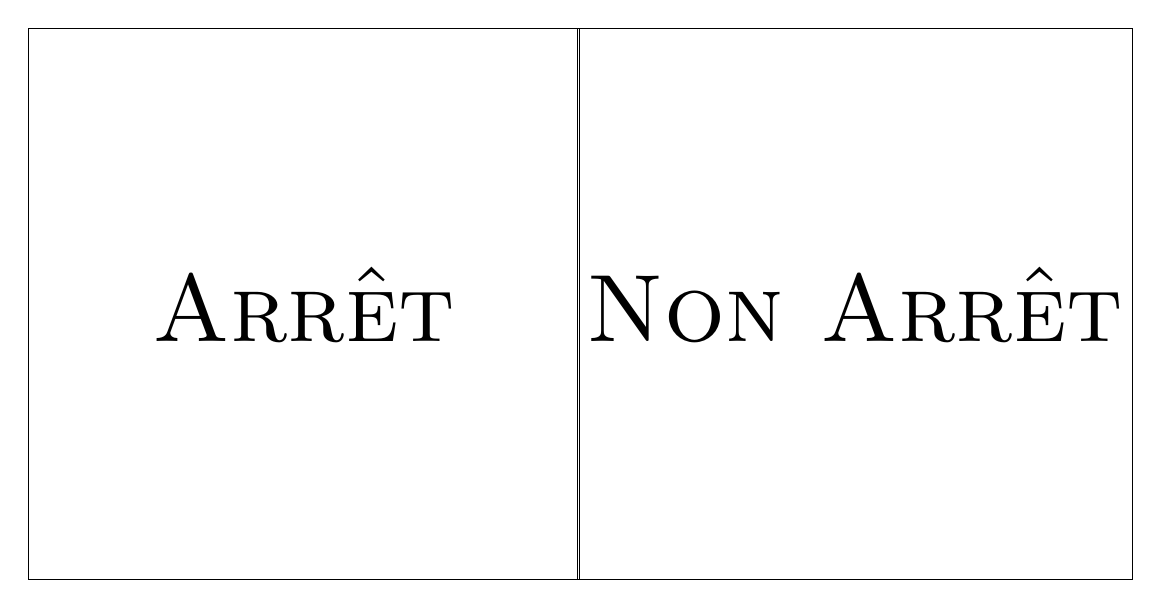
\begin{tikzpicture}
  \node[draw, rectangle, black, minimum width = 7 cm, minimum height =
  7 cm] at (0,0) {\scalebox{2}{\LARGE{\textsc{Arrêt}}}};

  \node[draw, rectangle, black, minimum width = 7 cm, minimum height =
  7 cm] at (7 cm,0) {\scalebox{2}{\LARGE{\textsc{Non Arrêt}}}};
\end{tikzpicture}


\scalebox{0.4}{
  \begin{tabular}{cc}
    % % \begin{figure}[h!]
    % %   \centering
    \resizebox{.5\textwidth}{!}{

    \begin{scratch}
      \blockinit{quand \v{E1} est présent}
      \blockvariable{mettre \v{S1} à \v{E1}}
      \blockvariable{mettre \v{S2} à \v{E1}}
%      \blockstop{stop}
    \end{scratch}
    }
    &
      \begin{minipage}{0.5 \textwidth}
        \vspace{8 cm}
        \hfill \scalebox{2}{\LARGE{\textsc{Photocopie}}} \hfill~
      \end{minipage}
  \end{tabular}
}


\scalebox{0.4}{
  \begin{tabular}{cc}
    % % \begin{figure}[h!]
    % %   \centering
    \resizebox{.5\textwidth}{!}{

    \begin{scratch}
      \blockinit{quand \v{E1} est présent}
      \blockvariable{mettre \v{S1} à \v{E1}}
      \blockvariable{mettre \v{S2} à \v{E1}}
%      \blockstop{stop}
    \end{scratch}
    }
    &
      \begin{minipage}{0.5 \textwidth}
        \vspace{8 cm}
        \hfill \scalebox{2}{\LARGE{\textsc{Photocopie}}} \hfill~
      \end{minipage}
  \end{tabular}
}


\scalebox{0.4}{
  \begin{tabular}{cc}
    % % \begin{figure}[h!]
    % %   \centering
    \resizebox{.5\textwidth}{!}{

    \begin{scratch}
      \blockinit{quand \v{E1} est présent}
      \blockvariable{mettre \v{S1} à \v{E1}}
      \blockvariable{mettre \v{S2} à \v{E1}}
%      \blockstop{stop}
    \end{scratch}
    }
    &
      \begin{minipage}{0.5 \textwidth}
        \vspace{8 cm}
        \hfill \scalebox{2}{\LARGE{\textsc{Photocopie}}} \hfill~
      \end{minipage}
  \end{tabular}
}

\end{document}

%% \pagebreak


%% \begin{tikzpicture}
%%   \node[draw, rectangle, black, minimum width = 6 cm, minimum height =
%%   6 cm] at (0,0) {\scalebox{10}{\LARGE{\textsc{0}}}};

%%   \node[draw, rectangle, black, minimum width = 6 cm, minimum height =
%%   6 cm] at (6 cm,0) {\scalebox{10}{\LARGE{\textsc{1}}}};

%%   \node[draw, rectangle, black, minimum width = 6 cm, minimum height =
%%   6 cm] at (12 cm,0) {\scalebox{10}{\LARGE{\textsc{2}}}};

%%   \node[draw, rectangle, black, minimum width = 6 cm, minimum height =
%%   6 cm] at (0,-6cm) {\scalebox{10}{\LARGE{\textsc{3}}}};

%%   \node[draw, rectangle, black, minimum width = 6 cm, minimum height =
%%   6 cm] at (6 cm,-6cm) {\scalebox{10}{\LARGE{\textsc{4}}}};

%%   \node[draw, rectangle, black, minimum width = 6 cm, minimum height =
%%   6 cm] at (12 cm,-6cm) {\scalebox{10}{\LARGE{\textsc{6}}}};

%%   \node[draw, rectangle, black, minimum width = 6 cm, minimum height =
%%   6 cm] at (0 cm,-12cm) {\scalebox{10}{\LARGE{\textsc{6}}}};

%%   \node[draw, rectangle, black, minimum width = 6 cm, minimum height =
%%   6 cm] at (6 cm,-12cm) {\scalebox{10}{\LARGE{\textsc{7}}}};

%%   \node[draw, rectangle, black, minimum width = 6 cm, minimum height =
%%   6 cm] at (12 cm,-12cm) {\scalebox{10}{\LARGE{\textsc{8}}}};

%%   \node[draw, rectangle, black, minimum width = 6 cm, minimum height =
%%   6 cm] at (0 cm,-18cm) {\scalebox{10}{\LARGE{\textsc{9}}}};

%%   \node[draw, rectangle, black, minimum width = 6 cm, minimum height =
%%   6 cm] at (6 cm,-18cm) {\scalebox{10}{\LARGE{\textsc{1\hspace{-0.15em}0}}}};

%%   \node[draw, rectangle, black, minimum width = 6 cm, minimum height =
%%   6 cm] at (12 cm,-18cm) {\scalebox{10}{\LARGE{\textsc{1\hspace{-0.15em}1}}}};
%% \end{tikzpicture}

%% \end{document}

